%%=============================================================================
%% Methodologie
%%=============================================================================


\chapter{\IfLanguageName{dutch}{Methodologie}{Methodology}}%
\label{ch:methodologie}

%% TODO: In dit hoofstuk geef je een korte toelichting over hoe je te werk bent
%% gegaan. Verdeel je onderzoek in grote fasen, en licht in elke fase toe wat
%% de doelstelling was, welke deliverables daar uit gekomen zijn, en welke
%% onderzoeksmethoden je daarbij toegepast hebt. Verantwoord waarom je
%% op deze manier te werk gegaan bent.
%% 
%% Voorbeelden van zulke fasen zijn: literatuurstudie, opstellen van een
%% requirements-analyse, opstellen long-list (bij vergelijkende studie),
%% selectie van geschikte tools (bij vergelijkende studie, "short-list"),
%% opzetten testopstelling/PoC, uitvoeren testen en verzamelen
%% van resultaten, analyse van resultaten, ...
%%
%% !!!!! LET OP !!!!!
%%
%% Het is uitdrukkelijk NIET de bedoeling dat je het grootste deel van de corpus
%% van je bachelorproef in dit hoofstuk verwerkt! Dit hoofdstuk is eerder een
%% kort overzicht van je plan van aanpak.
%%
%% Maak voor elke fase (behalve het literatuuronderzoek) een NIEUW HOOFDSTUK aan
%% en geef het een gepaste titel.

Het doel van dit onderzoek is het identificeren van de meest geschikte pipeline voor de automatisering van het orderproces van een website naar 3D-geprinte producten. Dit proces zal iteratief verlopen, met fasen die zich richten op onderzoek, evaluatie, en prototyping. Elke fase heeft specifieke doelstellingen, deliverables en deadlines. Ook is het de bedoeling dat deze pipeline zal draaien op Mac en Windows.
\vspace{2em}

\textbf{Fase 1: Literatuurstudie}\\
\textbf{(Deadline: 07 maart 2025)}\\\\
In deze fase wordt er literatuuronderzoek gedaan naar bestaande oplossingen en pipelines die gebruikt kunnen worden voor de automatisering van het orderproces. Dit omvat een analyse van tools zoals Python, integraties met de Shopify API, en printbeheer API's zoals Bambu Studio. De deliverable voor deze fase is een lijst met mogelijke pipelines en tools die geschikt zouden kunnen zijn voor dit project, inclusief voor- en nadelen van elke optie.
\vspace{2em}

\textbf{Fase 2: Proof-of-Concept (PoC)}\\
\textbf{(Deadline: 4 april 2025)}\\\\
Op basis van de literatuurstudie worden meerdere pipelines geselecteerd en getest door een PoC op te zetten voor elke gekozen oplossing. Dit zal helpen om de haalbaarheid van de verschillende pipelines te testen. De PoC zal een order ontvangen via de Shopify API en doorsturen naar de Bambu Studio API. De technische haalbaarheid van elke pipeline wordt geëvalueerd om te bepalen welke het beste presteert.
\vspace{1em}

\textbf{Fase 3: Testen en Optimalisatie van de Geselecteerde Pipeline}\\
\textbf{(Deadline: 25 april 2025)}\\\\
In deze fase wordt één pipeline verder uitgewerkt op basis van de voorlopige evaluaties. Hoewel nog geen definitieve keuze gemaakt is, zal de focus liggen op de oplossing die tijdens de proof-of-concept het meest beloftevol bleek. De andere pipelines worden voorlopig niet verder onderzocht.
\vspace{2em}
De gekozen pipeline wordt grondig getest onder verschillende omstandigheden, zoals foutscenario’s, verhoogde belasting en gelijktijdige bestellingen. Daarnaast worden eerste optimalisaties doorgevoerd om de betrouwbaarheid, foutafhandeling en prestaties te verbeteren. Om zo tot een beter eindresultaat te komen.
\\\\
\textbf{Testscenario’s omvatten onder andere:}
\begin{itemize}
    \item Wat gebeurt er als een G-code bestand niet correct verzonden wordt?
    \item Hoe wordt een printfout opgevangen?
    \item Hoe verloopt het gecontroleerd beëindigen van een printproces?
    \item Wat gebeurt er bij meerdere orders tegelijk?
\end{itemize}

\vspace{1em}
\textbf{Optimalisatie-aspecten:}
\begin{itemize}
    \item Verbeteren van foutdetectie en logging.
    \item Verkennen van parallelle printmogelijkheden op langere termijn.
    \item Opruimen van overbodige afhankelijkheden in het ontwikkelproces.
\end{itemize}

\vspace{1em}
\textbf{Dit is de verwachte lijst van Tools:}\\
\begin{itemize}
    \item Python: voor het bouwen van de pipeline en het uitvoeren van API-aanroepen.
    \item Shopify API en Bambu Studio API: om orders te ontvangen en printopdrachten door te sturen.
    \item GitHub: voor versiebeheer van de code en documentatie.
    \item Postman: voor het testen van API-aanroepen tijdens de ontwikkeling.
    \item 3D-printer Bambu Lab X1C: voor het fysiek testen van het printproces.
    \item Verschillende pipelinetools: voor het opzetten en automatiseren van de integratie tussen de verschillende onderdelen van het systeem.
\end{itemize}

\vspace{1em}
\textbf{Dit is de verwachte lijst van functionele vereisten voor de applicatie:}
\\\\
Deze lijst is opgesteld op basis van de initiële projectdoelen en inzichten uit de literatuurstudie. Tijdens de Proof-of-Concept (Fase 2) en testfase (Fase 3) zullen deze vereisten geëvalueerd en indien nodig bijgesteld worden op basis van praktische haalbaarheid en testresultaten.
\\\\
\begin{itemize}
    \item \textbf{MUST}
    \begin{itemize}
        \item Order moet kunnen opgehaald worden  via de API.
        \item Juiste file moet kunnen opgehaald worden.
        \item Printopdracht moet kunnen gestart worden via de API.
    \end{itemize}
    \item \textbf{SHOULD}
    \begin{itemize}
        \item Communicatie naar eigenaar dat print gelsaagd is.
    \end{itemize}
    \item \textbf{COULD}
    \begin{itemize}
        \item Als meerdere orders binnenkomen deze samen plaatsen op het printbed indien mogelijk.
    \end{itemize}
\end{itemize}

\vspace{1em}
\textbf{Planning en deliverables}

\begin{itemize}
    \item Gemaakte flowchart
    
    \begin{figure}[H]  % Use [H] to prevent floating
        \centering
        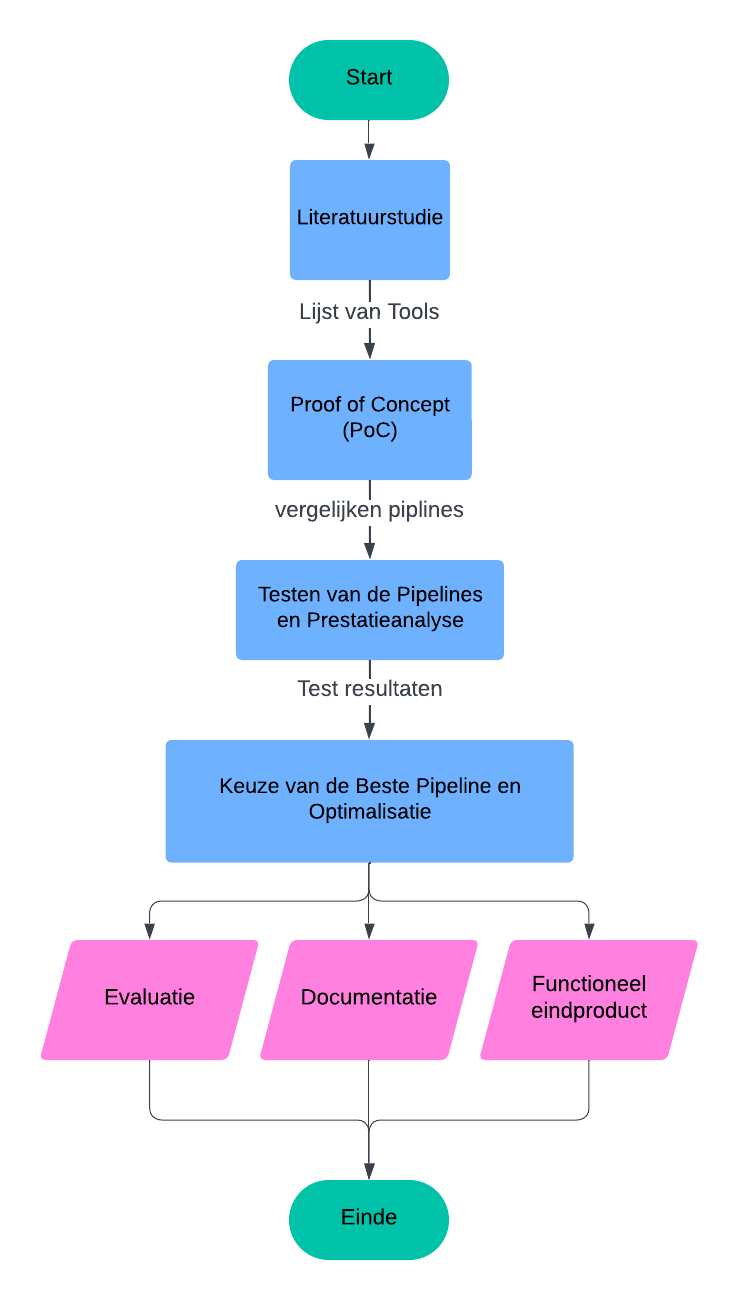
\includegraphics[width=0.5\textwidth]{Flowchart.png}  % Adjust width if necessary
        \caption{Flowchart van verschillende fasen en deliverables van de bachelorproef.}
        \label{fig:flowchart}  % Label for referencing
    \end{figure}
    
    \item Gemaakte Gantt chart.
    
    % Second figure: The Gantt Chart
    \begin{figure}[H]  % Use [H] to prevent floating
        \centering
        \resizebox{\textwidth}{!}{%
            \begin{ganttchart}[
                vgrid,
                hgrid,
                x unit=0.1cm,
                time slot format=isodate,
                compress calendar
                ]{2025-02-01}{2025-05-30}
                
                \gantttitlecalendar{year, month=name} \\
                
                % Fase 1: Literatuurstudie
                \ganttbar[
                progress=100,
                name=litstudie
                ]{Fase 1: Literatuurstudie}{2025-02-01}{2025-02-20} \\
                
                % Fase 2: Proof of Concept (PoC)
                \ganttbar[
                progress=0,
                name=poc
                ]{Fase 2: Proof-of-Concept}{2025-02-21}{2025-04-04} \\
                
                % Fase 3: Experimenten en Testen
                \ganttbar[
                progress=0,
                name=testen
                ]{Fase 3: Testen van de Pipelines en Prestatieanalyse}{2025-04-05}{2025-04-18} \\
                
                % Fase 4: Iteratieve Ontwikkeling en Optimalisatie
                \ganttbar[
                progress=0,
                name=optimalisatie
                ]{Fase 4: Keuze van de Beste Pipeline en Optimalisatie}{2025-04-19}{2025-04-25} \\
                
            \end{ganttchart}
        }
        \caption{Project Planning Gantt Chart}
        \label{fig:ganttchart}  % Label for referencing
    \end{figure}
\end{itemize}

\chapter{\IfLanguageName{dutch}{Proof-of-Concept}{Proof-of-Concept}}%
\label{ch:poc}

\section{Doel van deze fase}
Het doel van deze fase was het opzetten van alle werkende piplines tussen de webshop en de 3D-printer, ter validatie van de gekozen tools en technieken.

\section{Technische opstelling}
\begin{itemize}
    \item \textbf{Webshop:} Shopify met Webhook-integratie voor automatische orderdetectie.
    \item \textbf{3D-printer:} Creality Ender 3, aangestuurd via Raspberry Pi met MainsailOS + Moonraker API.
    \item \textbf{Communicatie:} Curl-commando’s naar Moonraker API voor slicen, uploaden en starten van printopdrachten.
    \item \textbf{Netwerktoegang:} Ngrok gebruikt om tijdelijk toegang te verlenen tot lokale services.
\end{itemize}

\section{Opmerkingen bij Bambu Lab Printer}
Initieel was het de bedoeling om de Bambu Lab X1C te gebruiken in combinatie met de Bambu Studio API. Door een software-update werd externe aansturing echter onmogelijk gemaakt zonder hun gesloten software. Daarom werd er overgeschakeld naar een open-source en lokaal beheersbare setup.

\section{CI/CD Tooling Evaluatie}
Om het automatiseringsproces te beheren en te testen, werden verschillende CI/CD tools onderzocht. Hieronder volgt een overzicht van de evaluatie:

\subsection{Geteste Tools}

\subsubsection{Jenkins (via Docker)}
\begin{itemize}
    \item \textbf{Voordelen:}
    \begin{itemize}
        \item Volledig lokaal hostbaar.
        \item Uitgebreide configuratiemogelijkheden via plugins.
        \item Volledige controle over netwerk en opslag.
        \item Geen problemen met authentificatie naar Moonraker.
    \end{itemize}
    \item \textbf{Nadelen:}
    \begin{itemize}
        \item Iets complexere setup (via Docker).
    \end{itemize}
\end{itemize}

\subsubsection{GitHub Actions}
\begin{itemize}
    \item \textbf{Voordelen:}
    \begin{itemize}
        \item Eenvoudige YAML-configuraties.
    \end{itemize}
    \item \textbf{Nadelen:}
    \begin{itemize}
        \item Enkel cloud-based, dus geen toegang tot lokaal netwerk of printers. (wel met ngrok)
        \item Vereist publieke poorten en authentificatie naar Moonraker.
        \item Veiligheidsrisico’s bij netwerktoegang.
    \end{itemize}
\end{itemize}

\subsubsection{GitLab CI/CD}
\begin{itemize}
    \item \textbf{Voordelen:}
    \begin{itemize}
        \item YAML-configuratie idem aan die van github actions met kleine aanpassingen.
        \item Self host gitlab runner dus kan lokaal gedraaid worden.
    \end{itemize}
    \item \textbf{Nadelen:}
    \begin{itemize}
        \item Vereist publieke poorten en authentificatie naar Moonraker. (online methode)
        \item Veiligheidsrisico’s bij netwerktoegang. (online methode)
        \item Maar 400 CI/CD minuten per maand.
    \end{itemize}
\end{itemize}

\subsection{Niet Geteste Tools}
Omwille van tijd door de bambulab update en kosten dat nodig zijn als je deze gebruikt op lange termijn, werden onderstaande tools niet verder onderzocht:
\begin{itemize}
    \item Bitbucket Pipelines
    \item Google Cloud Build
\end{itemize}

\section{PoC 1: Jenkins integratie}
\subsection{Verwerking van een Order met Jenkins}
\begin{enumerate}
    \item Shopify stuurt via Webhook een order door.
    \item Jenkins pipeline wordt getriggerd door de webhook.
    \item De juiste G-code wordt geselecteerd in de pipeline.
    \item Commando’s worden via curl doorgestuurd naar Moonraker:
    \begin{itemize}
        \item \texttt{G28} commando om te 'homen'
        \item Upload naar MainsailOS
        \item Start van de printopdracht
    \end{itemize}
\end{enumerate}

\subsection{Stappenplan Uitgevoerde Oplossing}

Onderstaande stappen beschrijven de volledige opzet- en uitvoeringsproces van de pipeline waarbij een Shopify-webhook via Jenkins een 3D-printopdracht start op een Raspberry Pi met MainsailOS en Moonraker.

\subsubsection{Stap 1: Installaties en Voorbereidingen}
\begin{enumerate}
    \item Maak een \textbf{Shopify-winkel} aan.
    \item Installeer \textbf{Docker} op je lokale machine.
    \item Maak in Docker een aangepaste Jenkins-container aan, dit commando zorgt ervoor dat de container met het lokaal netwerk kan communiceren en dat er een volume aan gekoppeld  wordt:
    \begin{lstlisting}[language=bash, caption=Docker commando voor Jenkins met volume en poorten]
        docker run -d -p 8080:8080 -p 50000:50000 -v "D:\_3D_print_\Webshop:/var/jenkins_home" --name jenkins-met-backup jenkins-met-wijzigingen:custom
    \end{lstlisting}
    \item Installeer \textbf{Ngrok} om publieke toegang te voorzien naar je Jenkins-container.
    \item Start Jenkins en kopieer het initiële admin-wachtwoord uit de Docker terminal.
    \item Maak een admin account aan in de Jenkins UI.
    
    \item Installeer noodzakelijke Jenkins plugins:
    \begin{itemize}
        \item \texttt{Generic Webhook Trigger Plugin}
    \end{itemize}
    \item Open poort 8080 via Ngrok:
    \begin{lstlisting}[language=bash]
        ngrok http 8080
    \end{lstlisting}

\end{enumerate}

\vspace{0.5em}
\begin{figure}[H]
    \centering
    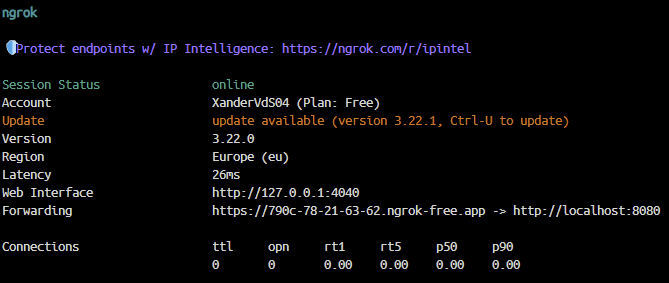
\includegraphics[width=1\linewidth]{foto's/ngrokWithJenkins.png}
    \caption{Docker Jenkins Container + Ngrok terminal output.}
    \label{fig:Ngrok-terminal}
\end{figure}

\subsubsection{Stap 2: Webhook Instellen in Shopify}
\begin{enumerate}
    \item Navigeer in Shopify naar \texttt{Instellingen > Meldingen > Webhooks}.
    \item Voeg een nieuwe webhook toe bij ``Bestelling aangemaakt''.
    \item Stel de webhook-URL in als volgt:
    \begin{lstlisting}[language=text]
        https://<jouw-ngrok-url>/generic-webhook-trigger/invoke?token=shopify-jenkins-trigger
    \end{lstlisting}
    \item Kies als indeling: \texttt{JSON}.
\end{enumerate}

\vspace{0.5em}
\begin{figure}[H]
    \centering
    
\includegraphics[width=1\linewidth]{foto's/ShopifyWebhookConfig.png}
    \caption{Shopify webhook-configuratie.}
    \label{fig:Shopify-Webhook-configuratie}
\end{figure}

\subsubsection{Stap 3: Aanmaken Jenkins Pipeline}
\begin{enumerate}
    \item Maak een nieuw Pipeline-project aan in Jenkins.
    \item Koppel het project aan een GitHub-repository.
    \item Voeg een \texttt{Jenkinsfile} toe in de repo met volgende inhoud:

\paragraph*{Stap 1: Shopify trigger naar Jenkins}

Een \texttt{Generic Webhook Trigger} plugin wordt gebruikt in Jenkins om inkomende bestellingen te detecteren. Hieronder zie je het deel van de configuratie dat de trigger mogelijk maakt:

\begin{lstlisting}[language=groovy, caption=Webhook-trigger configuratie in Jenkinsfile]
    triggers {
        GenericTrigger(
        genericVariables: [
        [key: 'order_id', value: '$.id'],
        [key: 'product_names', value: '$.line_items[*].name', expressionType: 'JSONPath']
        ],
        token: 'shopify-jenkins-trigger'
        )
    }
\end{lstlisting}

\paragraph*{Stap 2: Controle van het bestandsvolume}

Vooraleer een printopdracht wordt verstuurd, wordt nagegaan of het juiste G-code bestand bestaat in de Jenkins container (via een Docker volume gekoppeld aan de host).

\begin{lstlisting}[language=groovy, caption=Controle van Jenkins volume]
    stage('Check File System') {
        steps {
            sh 'ls -la /var/jenkins_home'
        }
    }
\end{lstlisting}

\paragraph*{Stap 3: Informatie over de bestelling loggen}

Bij het ontvangen van de bestelling loggen we de producten zodat we later kunnen debuggen of analyseren wat er is binnengekomen.

\begin{lstlisting}[language=groovy, caption=Debugging van de ontvangen productnamen]
    stage('Debug Bestelling') {
        steps {
            echo "Ontvangen productnamen: ${env.product_names}"
        }
    }
\end{lstlisting}

\paragraph*{Stap 4: Voorbereiding van het G-code bestand}

We selecteren één product en controleren of het bijhorende .gcode bestand klaarstaat om geprint te worden:

\begin{lstlisting}[language=groovy, caption=Controleren van G-code beschikbaarheid]
    stage('Prepare G-code') {
        steps {
            script {
                def order_name = env.product_names.replaceAll("[\\[\\]\" ]", "").split(",")[0]
                def gcodeFilePath = "/var/jenkins_home/${order_name}.gcode"
                if (!fileExists(gcodeFilePath)) {
                    error "G-code niet gevonden: ${gcodeFilePath}"
                }
            }
        }
    }
\end{lstlisting}

\paragraph*{Stap 5: Verzenden van de printopdracht}

Zodra alles correct is voorbereid, worden via CURL-commando’s drie instructies naar de printer gestuurd:

\begin{enumerate}
    \item \textbf{G28} om de printer te 'homing'.
    \item Upload van het G-code bestand.
    \item Starten van het printproces.
\end{enumerate}

\begin{lstlisting}[language=groovy, caption=Starten van het printproces via curl]
    stage('Start Print') {
        steps {
            script {
                sh '''curl -X POST .../printer/gcode/script -d '{"script": "G28"}' '''
                sh '''curl -X POST .../server/files/upload -F "file=@..." '''
                sh '''curl -X POST .../printer/print/start -d '{"filename": "..."}' '''
            }
        }
    }
\end{lstlisting}

\subsubsection{Stap 4: Bestandenstructuur en G-code}
\begin{itemize}
    \item De G-code bestanden worden lokaal bewaard in de Jenkins volume map: \texttt{/var/jenkins\_home/}.
    \item De naam van het bestand moet overeenkomen met het ontvangen product via Shopify.
\end{itemize}

\vspace{0.5em}
\begin{figure}[H]
    \centering
    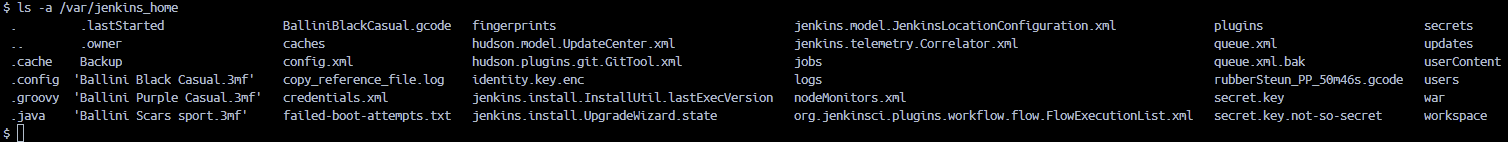
\includegraphics[width=1\linewidth]{foto's/JenkinsHome.png}
    \caption{bestand in map \texttt{jenkins\_home} zichtbaar via Jenkins console voor .3mf.}
    \label{fig:Jenkins_home}
\end{figure}

\subsubsection{Stap 5: Printer Instellingen}
\begin{itemize}
    \item Raspberry Pi draait MainsailOS met Moonraker.
    \item Printer is lokaal bereikbaar via IP: \texttt{192.168.1.100:7125}.
    \item Curl-commando’s sturen G-code naar de printer.
    \item Volgorde: Homen met \texttt{G28} → uploaden → print starten.
\end{itemize}

\vspace{0.5em}
\begin{figure}[H]
    \centering
    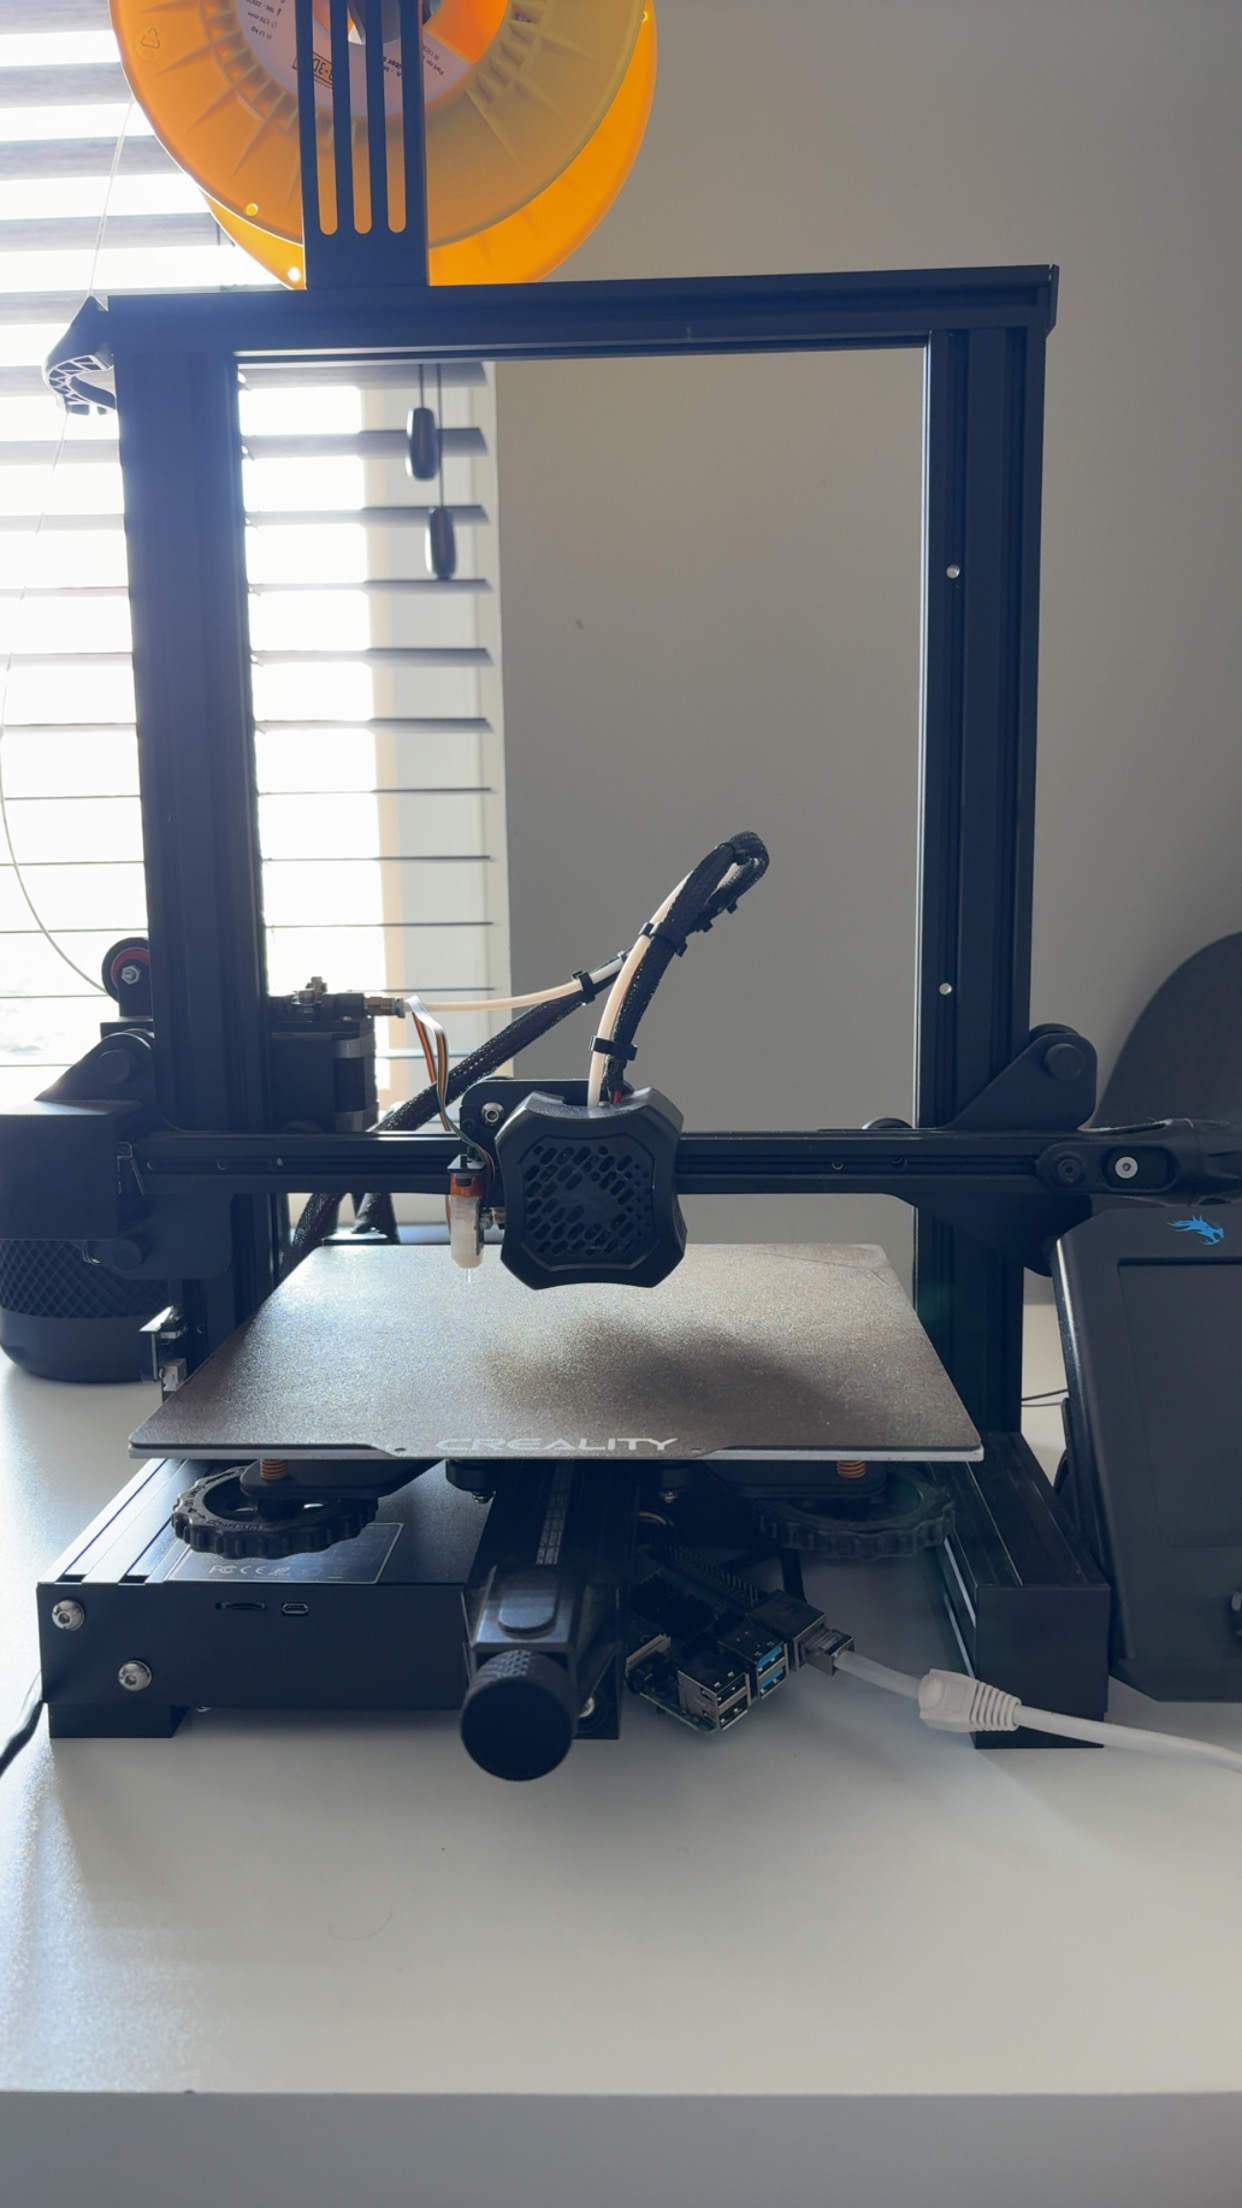
\includegraphics[width=0.3\linewidth]{foto's/Ender3WithRaspberryPi.JPG}
    \caption{Raspberry Pi + Ender 3 V2 setup.}
    \label{fig:3Dprinter}
\end{figure}

\section{PoC 2: GitHub Actions Pipeline integratie}

In deze tweede PoC werd een GitHub Actions pipeline gebruikt. In plaats van Jenkins generic trigger wordt er gebruikgemaakt van een Express-server die de webhook ontvangt en vervolgens een GitHub Action triggert.

\subsection{Verwerking van een Order met GitHub Actions}

\begin{enumerate}
    \item Een Express-server draait lokaal en ontvangt webhook-events van Shopify.
    \item Bij ontvangst van een nieuwe bestelling wordt via de GitHub API een \texttt{repository\_dispatch} event verstuurd.
    \item Een GitHub Actions pipeline luistert op dit event en verwerkt de bestelling.
    \item De juiste G-code wordt geüpload naar een 3D-printer via een Ngrok-tunnel naar de Moonraker API.
\end{enumerate}

\subsection{Stappenplan Uitgevoerde Oplossing}

\subsubsection{Stap 1: Installaties en Voorbereidingen}

\begin{itemize}
    \item Maak een \textbf{Shopify-winkel} aan.
    \item G-code bestanden opgeslagen in een submap van deze repo (\texttt{gcodes/}).
    \item Een werkende Moonraker setup op een Raspberry Pi met MainsailOS.
    \item Een \texttt{GITHUB\_TOKEN} environment variabele (persoonlijke access token met repo rechten).
\end{itemize}

\subsubsection{Stap 2: Webhook Server (Express)}

De Express-server ontvangt webhooks en stuurt een dispatch-event naar GitHub.

\begin{lstlisting}[language=javascript, caption=Webhook-server (gedeeltelijk weergegeven)]
    const express = require('express');
    const axios = require('axios');
    require('dotenv').config();
    
    const app = express();
    app.use(express.json());
    
    app.post('/shopify-webhook', async (req, res) => {
        const orderId = req.body.id;
        const productNames = req.body.line_items.map((item) => item.name);
        
        try {
            await axios.post(
            'https://api.github.com/repos///dispatches',
            {
                event_type: 'shopify-order',
                client_payload: {
                    order_id: orderId,
                    product_names: productNames[0],
                },
            },
            {
                headers: {
                    Authorization: token ${process.env.GITHUB_TOKEN},
                },
            }
            );
            res.status(200).send('GitHub Action triggered');
        } catch (error) {
            res.status(500).send('Fout bij triggeren van GitHub');
        }
    });
    
    app.listen(3000);
\end{lstlisting}

De token moet beschikbaar zijn in een \texttt{.env} bestand:

\begin{lstlisting}[language=bash, caption=.env bestand voorbeeld]
    GITHUB_TOKEN=ghp_jouwpersoneletokenhier
\end{lstlisting}

\subsubsection{Stap 3: Shopify Webhook Configuratie}

\begin{itemize}
    \item Ga naar \texttt{Instellingen > Meldingen > Webhooks} in Shopify.
    \item Voeg een webhook toe voor "Order created".
    \item Gebruik de volgende URL:
    \begin{lstlisting}[language=text]
        https:///shopify-webhook
    \end{lstlisting}
    \item Kies als formaat \texttt{JSON}.
\end{itemize}

\subsubsection{Stap 4: GitHub Actions Pipeline}

Bij ontvangst van een \texttt{repository\_dispatch} wordt deze pipeline uitgevoerd.

\begin{lstlisting}[language=yaml, caption=Shopify Order Print Pipeline (gedeeltelijk)]
    on:
    repository_dispatch:
    types: [shopify-order]
    
    jobs:
    print-job:
    runs-on: ubuntu-latest
    steps:
    - name: Checkout repository
    uses: actions/checkout@v4
    
      - name: Extract Order Info
    id: extract
    run: |
    echo "Product: ${{ github.event.client_payload.product_names }}"
    ... extractie- en bestandslogica ...
    
    - name: Upload & Start Print
    run: |
    curl -X POST .../printer/gcode/script -d '{"script": "G28"}'
    curl -X POST .../server/files/upload -F "file=@..."
    curl -X POST .../printer/print/start -d '{"filename": "..."}'
\end{lstlisting}

\subsubsection{Stap 5: Mappenstructuur en Bestandseisen}

\begin{itemize}
\item De map \texttt{gcodes/} in de GitHub repo bevat de benodigde \texttt{.gcode} bestanden.
\item De bestandsnamen moeten exact overeenkomen met de Shopify productnamen.
\end{itemize}

\begin{figure}[H]
    \centering
    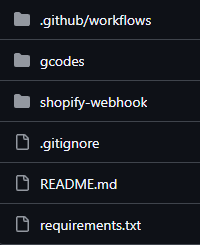
\includegraphics[width=0.3\linewidth]{foto's/Github/Schermafbeelding 2025-04-22 161449.png}
    \caption{mappenstructuur in de GitHub repository}
    \label{fig:Github_Repo}
\end{figure}

\subsubsection{Stap 6: Ngrok Setup}

Zorg ervoor dat zowel je Express-server als je Moonraker API extern bereikbaar zijn. Start Ngrok bijvoorbeeld als volgt:

\begin{lstlisting}[language=bash, caption=Ngrok tunnel starten voor Express]
ngrok http 3000
\end{lstlisting}

\begin{lstlisting}[language=bash, caption=Ngrok tunnel starten voor Moonraker]
ngrok http 7125
\end{lstlisting}

\begin{figure}[H]
    \centering
    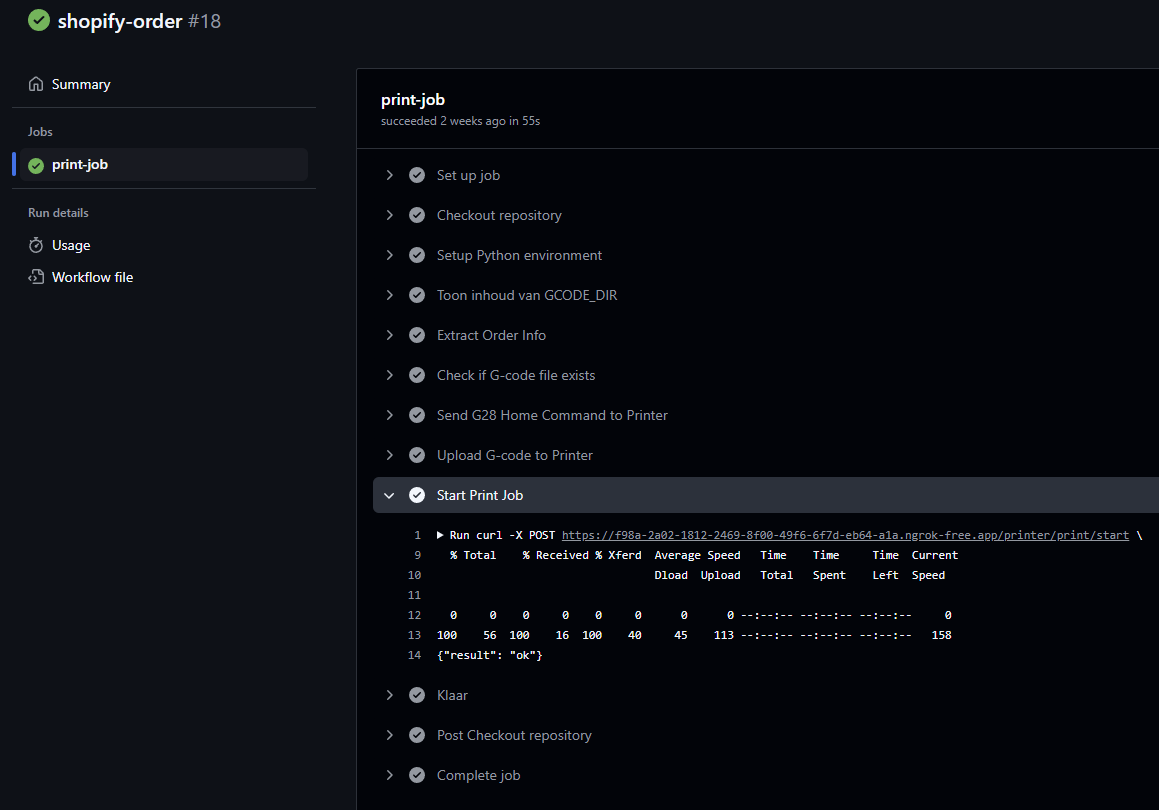
\includegraphics[width=1\linewidth]{foto's/Github/GithubPrintSucces.png}
    \caption{Voorbeeld van een succesvolle GitHub Actions run}
    \label{fig:Github_Succes}
\end{figure}

\section{Stappenplan PoC 3: GitLab CI/CD Integratie}

De derde en laatste PoC gebruikt GitLab CI/CD. Hierbij worden omgevingsvariabelen gebruikt en wordt een GitLab pipeline getriggerd via een API-call.

\subsection{Stappenplan Uitgevoerde Oplossing}

\subsubsection{Stap 1: Installaties en Voorbereidingen}
\begin{itemize}
    \item Maak een \textbf{Shopify-winkel} aan.
    \item Een publieke GitLab repository met een \texttt{.gitlab-ci.yml} bestand.
    \item Twee Ngrok-tunnels: één voor de webhook-server (indien gebruikt), één voor de printer.
    \item Een Raspberry Pi met MainsailOS en Moonraker geïnstalleerd.
    \item Een pipeline trigger token van GitLab.
\end{itemize}

\subsubsection{Stap 2: Webhook Setup of Directe Trigger}
Er zijn twee mogelijkheden om de pipeline te starten:
\begin{enumerate}
    \item \textbf{Via een Node.js Webhook Server} (zoals bij PoC 2): deze ontvangt de bestelling van Shopify en doet een POST-request naar de GitLab API.
    \item \textbf{Rechtstreeks in Shopify} bij het instellen van de webhook-URL:
    \begin{lstlisting}[language=text, caption=Voorbeeld GitLab trigger-URL]
        https://gitlab.com/api/v4/projects/<PROJECT_ID>/ref/master/trigger/pipeline?token=<JOUW_TOKEN>&variables[ORDER_ID]=123456&variables[PRODUCT_NAMES]=Ballini%20Black%20Casual
    \end{lstlisting}
\end{enumerate}

\subsubsection{Stap 3: Pipelineconfiguratie in GitLab}
Het volgende \texttt{.gitlab-ci.yml} bestand wordt gebruikt om de printopdracht uit te voeren:

\begin{lstlisting}[language=yaml, caption=.gitlab-ci.yml structuur (vereenvoudigd)]
    image: python:3.11-slim
    
    stages:
    - prepare
    - check
    - print
    
    variables:
    PRINTER_HOST: 192.168.1.100
    GCODE_DIR: ./gcodes
    
    before_script:
    - apt-get update && apt-get install -y curl
    - python -m venv venv
    - source venv/bin/activate
    - pip install -r requirements.txt
    
    print-job:
    stage: print
    script:
    - echo "Product: $PRODUCT_NAMES"
    - export ORDER_NAME=$(echo "$PRODUCT_NAMES" | sed 's/ //g' | cut -d',' -f1)
    - export GCODE_FILE="$GCODE_DIR/$ORDER_NAME.gcode"
    - test -f "$GCODE_FILE" || exit 1
    - curl -X POST <NGROK_URL>/printer/gcode/script -d '{"script": "G28"}'
    - curl -X POST <NGROK_URL>/server/files/upload -F "file=@$GCODE_FILE"
    - curl -X POST <NGROK_URL>/printer/print/start -d "{\"filename\": \"$ORDER_NAME.gcode\"}"
\end{lstlisting}

\subsubsection{Stap 4: Netwerk en Beveiliging}
\begin{itemize}
    \item Voor deze setup heb je idealiter twee aparte Ngrok-tunnels nodig:
    \begin{itemize}
        \item Eén om de printer aan te sturen via Moonraker.
        \item Eén voor een mogelijke Node.js server als tussenlaag (optioneel).
    \end{itemize}
    \item Aangezien meerdere Ngrok-tunnels tegelijk draaien, is een betaald Ngrok-abonnement vereist.
    \item Tokens en geheime variabelen zoals het GitLab trigger-token moeten worden beheerd via omgevingsvariabelen of GitLab CI/CD Secrets.
\end{itemize}

\subsubsection{Stap 5: Structuur en Bestanden}
\begin{itemize}
    \item De \texttt{.gcode} bestanden worden in de \texttt{gcodes/} map van de GitLab repository geplaatst.
    \item De bestandsnaam moet overeenkomen met het product dat Shopify doorstuurt (zonder spaties of speciale tekens).
    \item \texttt{requirements.txt} bevat eventuele Python dependencies voor extra verwerking (optioneel).
\end{itemize}

\begin{figure}[H]
    \centering
    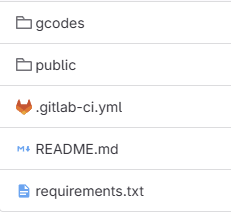
\includegraphics[width=0.3\linewidth]{foto's/Gitlab/folder.png}
    \caption{mappenstructuur in de GitLab repository}
    \label{fig:GitLab_Repo}
\end{figure}

\section{Afweging .py-scripts vs Curl}
Tijdens de PoC is gebleken dat het gebruik van rechtstreekse \texttt{curl}-commando’s eenvoudiger en sneller resultaat gaf dan Python-scripts met externe libraries zoals \texttt{moonrakerpy}. Hierdoor werd gekozen om tijdens de PoC te werken met directe API-aanroepen.

\section{Afsluitende Opmerkingen}
\begin{itemize}
    \item Niet alle packages in \texttt{requirements.txt} werden effectief gebruikt (zelf geen bij Jenkins).
    \item Voor productie is het aangeraden om Jenkins lokaal op een Raspberry Pi te hosten i.p.v. via Ngrok.
    \item Curl biedt betrouwbaardere controle tijdens testen dan afhankelijkheden van externe libraries.
\end{itemize}

\section{Besluit}
Op basis van de uitgevoerde tests is \textbf{Jenkins} geselecteerd als meest geschikte tool voor verdere uitwerking. Belangrijke redenen zijn:
\begin{itemize}
    \item Volledig lokaal beheer.
    \item Flexibiliteit en uitbreidbaarheid.
    \item Geen externe afhankelijkheden of veiligheidsrisico’s.
\end{itemize}

Er is beslist om de Jenkins-oplossing verder te optimaliseren in de volgende fase van het project.

\chapter{\IfLanguageName{dutch}{Testen en Prestatieanalyse}{Testing and Performance Analysis}}%
\label{ch:test-en-prestatie}

\subsection{Doel}
In deze fase werd de Jenkins-oplossing onderworpen aan een reeks functionele en foutgebaseerde testscenario’s. Het doel was om de betrouwbaarheid, foutafhandeling en prestaties van de pipeline te evalueren binnen realistische omstandigheden.

\subsection{Testscenario’s}
\begin{itemize}
    \item Wat gebeurt er als een G-code bestand niet gevonden wordt?
    \item Hoe wordt gereageerd op printfouten of onderbrekingen tijdens het proces?
    \item Wat gebeurt er bij stroomuitval van de printer of het systeem?
    \item Hoe gaat het systeem om met meerdere bestellingen kort na elkaar?
\end{itemize}

\subsection{Resultaten}
\begin{itemize}
    \item De pipeline bevat een controle op de aanwezigheid van het benodigde G-code bestand in het Jenkins-bestandssysteem:
    \begin{lstlisting}[language=groovy]
        if (!fileExists(lokaalPad)) {
            error "❌ G-code bestand niet gevonden: ${lokaalPad}"
        }
    \end{lstlisting}
    Indien het bestand niet gevonden wordt, faalt de job correct met een duidelijke foutmelding.
    
    \item Tijdens het printen wordt de status van de printer opgevolgd:
    \begin{lstlisting}[language=groovy]
        def statusJson = sh(script: "curl -s ${env.PRINTER_URL}/api/job", returnStdout: true)
        def status = new groovy.json.JsonSlurperClassic().parseText(statusJson)
        def state = status?.state
        if (state == "Error") {
            error "❌ Fout opgetreden tijdens printen!"
        }
    \end{lstlisting}
    Bij fouten of onverwachte states zoals \texttt{Error} wordt de pipeline correct afgebroken.
    
    \item Bij stroomuitval of verlies van netwerkverbinding reageert de pipeline met een time-out of een HTTP-error. De pipeline blijft hierdoor hangen of faalt met een foutcode. Dit werd als logisch gedrag beschouwd, al kan de foutafhandeling verder verbeterd worden met notificaties (zie verder).
    
    \item Bestellingen met meerdere producten worden correct afgehandeld via sequentiële verwerking in één build:
    \paragraph{Verwerking per product met statuscontrole}
    
    Een sterke eigenschap van de pipeline is dat elke productlijn afzonderlijk verwerkt wordt binnen één webhookbuild. De pipeline controleert per product:
    
    \begin{itemize}
        \item Of het G-code bestand lokaal aanwezig is.
        \item Of het al op de printer staat (via de Moonraker file list).
        \item Of upload nodig is.
        \item Of de printer gehomed is (G28).
        \item Of het printjob correct toegevoegd en gestart is.
        \item Of de job correct afgerond wordt (state check via API).
    \end{itemize}
    
    De volledige verwerking gebeurt in één `stage`, waarin een lijst producten (uit de Shopify-bestelling) doorlopen wordt. Dit zorgt voor duidelijke foutmeldingen en garandeert dat alle producten geprint zijn voordat de job als succesvol beschouwd wordt.
    
    \begin{lstlisting}[language=groovy, caption=Sequentiële verwerking per product]
        stage('Print per product') {
            steps {
                script {
                    def producten = env.product_names.replaceAll("[\\[\\]\" ]", "").split(",")
                    def printerFilesJson = sh(script: "curl -s ${env.PRINTER_URL}/server/files/list?root=gcodes", returnStdout: true)
                    def printerFiles = new groovy.json.JsonSlurperClassic().parseText(printerFilesJson)
                    
                    for (product in producten) {
                        def productNaam = product.trim()
                        def bestandNaam = "${productNaam}.gcode"
                        def lokaalPad = "/var/jenkins_home/${bestandNaam}"
                        
                        echo "\n🔧 Verwerken: ${productNaam}"
                        
                        if (!fileExists(lokaalPad)) {
                            error "❌ G-code bestand niet gevonden: ${lokaalPad}"
                        }
                        
                        def bestandBestaat = printerFiles.result.any { it.path == bestandNaam }
                        if (!bestandBestaat) {
                            echo "⬆️ Bestand ${bestandNaam} wordt geüpload..."
                            ...
                        }
                        
                        echo "🏠 Homing uitvoeren (G28)..."
                        ...
                        
                        echo "📨 Job toevoegen aan wachtrij: ${bestandNaam}"
                        ...
                        
                        echo "🚦 Starten van job queue..."
                        ...
                        
                        echo "⏳ Wachten op printvoltooiing van ${bestandNaam}..."
                        timeout(time: env.MAX_WAIT_MINUTES.toInteger(), unit: 'MINUTES') {
                            waitUntil {
                                def statusJson = sh(script: "curl -s ${env.PRINTER_URL}/api/job", returnStdout: true).trim()
                                def status = new groovy.json.JsonSlurperClassic().parseText(statusJson)
                                def state = status?.state
                                
                                echo "📡 Printerstatus: ${state}"
                                
                                if (state == "Error") {
                                    error "❌ Fout opgetreden tijdens printen!"
                                } else if (state == "Operational") {
                                    echo "✅ Print van ${bestandNaam} voltooid."
                                    return true
                                } else {
                                    sleep(time: 20, unit: 'SECONDS')
                                    return false
                                }
                            }
                        }
                    }
                }
            }
        }
    \end{lstlisting}
    
    Deze aanpak maakt het eenvoudig om foutafhandeling, logging en statuscontrole netjes te isoleren per product. Dankzij Jenkins' configuratie die gelijktijdige builds voorkomt (zoals de setting \texttt{Do not allow concurrent builds}), worden builds geserialiseerd. Dit zorgt ervoor dat elke bestelling afzonderlijk en volledig wordt afgehandeld, zonder interferentie van andere lopende jobs.
    
    Dit gedrag simuleert als het ware een wachtrij op het niveau van de bestellingen, terwijl per bestelling de interne producten in volgorde worden afgewerkt. Hierdoor is parallelle verwerking nog niet nodig en wordt race-conditions vermeden.
    
    
    \item Meerdere bestellingen kort na elkaar worden netjes in wachtrij geplaatst dankzij Jenkins' ingebouwde jobbeheer. In de jobconfiguratie werd geactiveerd dat builds niet gelijktijdig mogen starten ( “Do not allow concurrent builds”). Hierdoor wordt gewaarborgd dat slechts één build tegelijk actief is per project. Nieuwe webhooks worden wel meteen ontvangen, maar pas uitgevoerd als de vorige printtaak is afgerond.
\end{itemize}

\subsection{Timing: Van Bestelling tot Printstart}

Tijdens het testen werd ook de tijd gemeten tussen het ontvangen van een bestelling (via webhook) en het daadwerkelijke starten van het printproces. Gemiddeld bleek dit tussen de 45 en 50 seconden te liggen, afhankelijk van factoren zoals bestandsgrootte, wachttijd op printerstatus en netwerkvertraging. Deze tijd omvat:

\begin{itemize}
    \item Ontvangst en verwerking van de webhook.
    \item Parsing van de productinformatie.
    \item Controle op aanwezigheid van het G-code bestand.
    \item Eventuele upload naar de printer.
    \item Homing van de printer (G28).
    \item Toevoegen van de job aan de wachtrij.
    \item Starten van de printopdracht.
\end{itemize}

Deze korte reactietijd is geschikt voor prototyping en kleine oplages, waarbij snelheid belangrijk is en elke opdracht snel moet starten zonder handmatige tussenkomst.

\subsection{Schaalbaarheid: Wat bij Meerdere Printers?}

In de huidige configuratie is er slechts één printer gekoppeld per Jenkins-pipeline. Dit vereenvoudigt de foutafhandeling en statusopvolging, maar beperkt uiteraard de verwerkingssnelheid. Voor scenario’s met meerdere printers zijn er verschillende uitbreidingsopties:

\begin{itemize}
    \item \textbf{Parallelle Pipelines:} Per printer kan een aparte Jenkins-job opgezet worden, elk met een unieke printer-URL. Door gebruik te maken van Jenkins labels of agents, kunnen builds verdeeld worden over meerdere fysieke machines of containers.
    
    \item \textbf{Printerrouter:} Een centrale dispatcher (bijvoorbeeld een Node.js of Python microservice) kan inkomende bestellingen verdelen over beschikbare printers op basis van hun status (bijv. 'idle'). Dit systeem kan gekoppeld worden aan een queue, zoals RabbitMQ of Redis Streams, met logica voor load balancing.
    
    \item \textbf{Per-printer wachtrijen:} Elke printer krijgt zijn eigen wachtrij met eigen verwerkingslogica. Zo vermijd je race conditions en kunnen verschillende bestellingen onafhankelijk verwerkt worden.
    
    \item \textbf{Printercluster configuratie:} Indien Moonraker meerdere printers ondersteunt via aparte API-instances, kan een supervisorproces de status van elk endpoint monitoren en opdrachten toewijzen op basis van beschikbaarheid.
\end{itemize}

Voor een doe-het-zelf (DIY) opzet is het aan te raden klein te starten: met twee printers en één centrale webhookserver die het routeringsprobleem oplost. In een latere fase kan dit uitgebouwd worden met persistente queues en automatische foutafhandeling per printer.


\subsection{E-mail bij foutmelding (uitbreidbaar)}
Indien gewenst kan er een aparte foutmeldingsserver voorzien worden die bij een printfout automatisch een e-mail stuurt naar de beheerder. De pipeline kan via een eenvoudige HTTP-call deze server aanroepen bij fouten. De Express-mailserver kan er als volgt uitzien:

\begin{lstlisting}[language=javascript, caption=Express-server voor foutnotificatie per e-mail]
    const express = require('express');
    const nodemailer = require('nodemailer');
    const app = express();
    app.use(express.json());
    
    app.post('/notify', async (req, res) => {
        const { subject, message } = req.body;
        const transporter = nodemailer.createTransport({
            service: 'Gmail',
            auth: {
                user: 'jouwmail@gmail.com',
                pass: 'jouwappwachtwoord'
            }
        });
        
        try {
            await transporter.sendMail({
                from: '"Printmonitor" <jouwmail@gmail.com>',
                to: 'beheerder@voorbeeld.com',
                subject,
                text: message
            });
            res.sendStatus(200);
        } catch (err) {
            console.error(err);
            res.sendStatus(500);
        }
    });
    
    app.listen(4000, () => console.log('Notifier actief op poort 4000'));
\end{lstlisting}

In de Jenkins pipeline zou je bij een fout in de printerstatus een melding kunnen laten sturen zoals hieronder. Deze uitbreiding werd niet meer getest tijdens Fase 3.

\begin{lstlisting}[language=groovy]
    if (state == "Error") {
        sh """
        curl -X POST http://localhost:4000/notify \\
        -H "Content-Type: application/json" \\
        -d '{"subject":"Printerfout", "message":"Fout opgetreden bij printen van ${bestandNaam}."}'
        """
        error "❌ Fout opgetreden tijdens printen!"
    }
\end{lstlisting}

\subsection{Afsluitende Opmerkingen}
\begin{itemize}
    \item Niet alle packages uit \texttt{requirements.txt} werden effectief gebruikt.
    \item Voor productieomgevingen wordt aanbevolen om Jenkins permanent lokaal te draaien op een Raspberry Pi, in plaats van tijdelijk via Ngrok.
    \item De directe \texttt{curl}-aanpak bood meer controle en eenvoud vergeleken met externe bibliotheken zoals \texttt{moonrakerpy}.
    \item De configuratie van Jenkins voorkomt race conditions bij meerdere bestellingen, wat cruciaal is voor correcte uitvoering.
\end{itemize}

\subsection{Besluit Fase 3}
De Jenkins-pipeline bleek stabiel en robuust onder normale omstandigheden en bij gecontroleerde fouten. Door het verbod op gelijktijdige builds worden bestellingen veilig sequentieel verwerkt, wat een betrouwbare flow oplevert.





